\chapter*{Introduction}
\addcontentsline{toc}{chapter}{Introduction}
\markboth{Introduction}{Introduction}
\label{chap:introduction}

L’importance du système de recommandation pour Netflix.

\vspace{5mm}

\begin{figure}[htp]
  \centering
  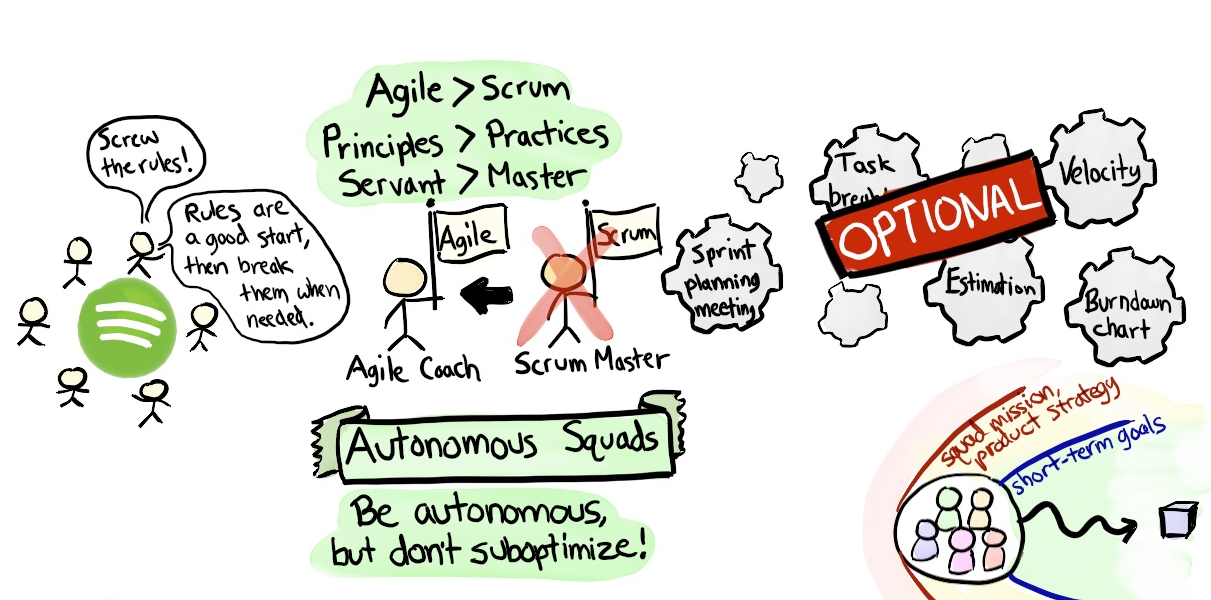
\includegraphics[width=95mm]{./src_img/agile_scrum}
  \caption{Organigramme du LRI.}
  \label{fig:uno}
\end{figure}

\vspace{5mm}

L'entreprise \textbf{Netflix} \supercite{NetflixNumerama} 

\vspace{5mm}



\vspace{5mm}

Les 11 et 12 avril \textit{Reed Hastings} présentait la stratégie de sa société \textbf{Netflix} pour les années à venir à la Cité du Cinéma, renommée \textit{Netflix City} pour l'occasion. Le symbole est fort et à l'image des changements que le service a apporté à l'industrie du divertissement et à notre manière de consommer les films et séries. Tout d'abord créé suite au mécontentement de son créateur à l'égard du service de location de films Blockbuster, alors en position de monopole, il a su se faire une place et créer par la suite un nouveau marché avec son service de vidéo à la demande\footnote{le cheval c'est trop génial}.

\vspace{5mm}
 